\documentclass[tikz,border=3mm]{standalone}
\usetikzlibrary{shapes.geometric, arrows}

\begin{document}
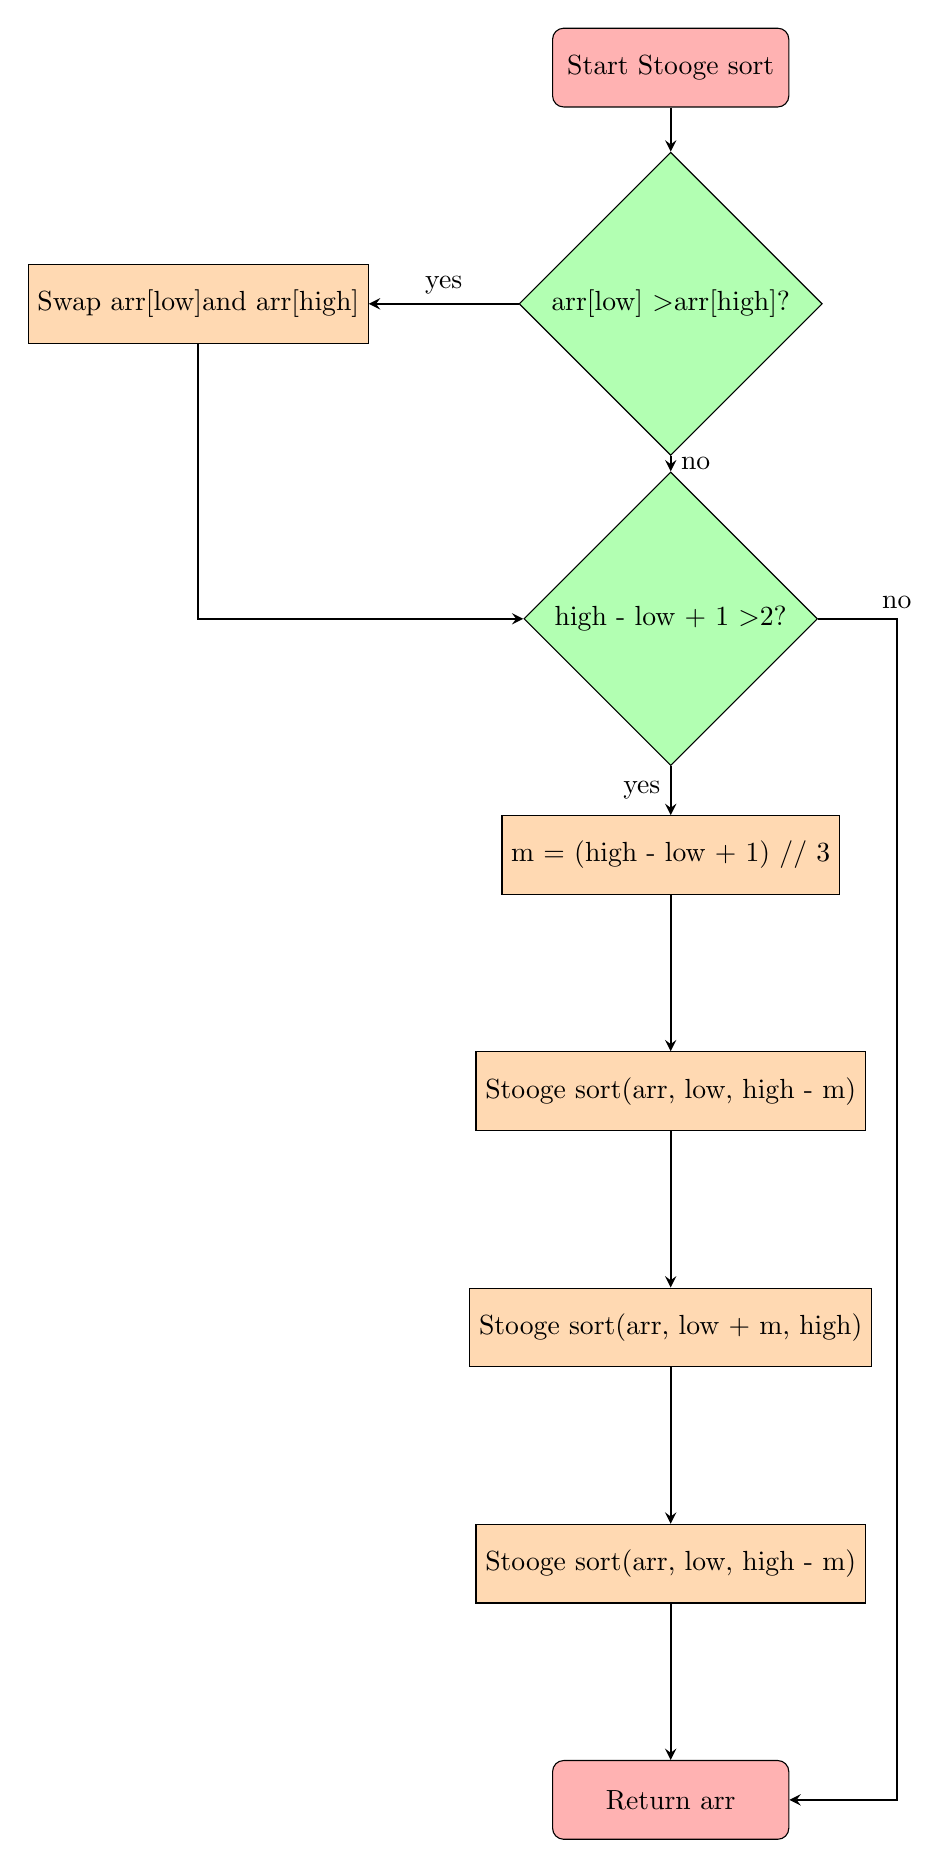
\begin{tikzpicture}[
    node distance=3cm,
    startstop/.style={rectangle, rounded corners, minimum width=3cm, minimum height=1cm, text centered, draw=black, fill=red!30},
    process/.style={rectangle, minimum width=3cm, minimum height=1cm, text centered, draw=black, fill=orange!30},
    decision/.style={diamond, minimum width=3cm, minimum height=1cm, text centered, draw=black, fill=green!30},
    arrow/.style={thick,->,>=stealth}
]

\node (start) [startstop] {Start Stooge sort};
\node (dec1) [decision, below of=start] {arr[low] \textgreater arr[high]?};
\node (swap) [process, left of=dec1, xshift=-3cm] {Swap arr[low]\\and arr[high]};
\node (dec2) [decision, below of=dec1, yshift=-1cm] {high - low + 1 \textgreater 2?};
\node (calc) [process, below of=dec2] {m = (high - low + 1) // 3};
\node (rec1) [process, below of=calc] {Stooge sort(arr, low, high - m)};
\node (rec2) [process, below of=rec1] {Stooge sort(arr, low + m, high)};
\node (rec3) [process, below of=rec2] {Stooge sort(arr, low, high - m)};
\node (stop) [startstop, below of=rec3] {Return arr};

% Arrows
\draw [arrow] (start) -- (dec1);
\draw [arrow] (dec1) -- node[anchor=south] {yes} (swap);
\draw [arrow] (swap) |- (dec2);
\draw [arrow] (dec1) -- node[anchor=west] {no} (dec2);
\draw [arrow] (dec2) -- node[anchor=east] {yes} (calc);
\draw [arrow] (calc) -- (rec1);
\draw [arrow] (rec1) -- (rec2);
\draw [arrow] (rec2) -- (rec3);
\draw [arrow] (rec3) -- (stop);
\draw [arrow] (dec2.east) -- ++(1,0) node[anchor=south] {no} |- (stop.east);

\end{tikzpicture}
\end{document}